\section{Results}
\label{sec-results}
\input graphsize_table

%\begin{figure*}[t]
%       \begin{center}
%                       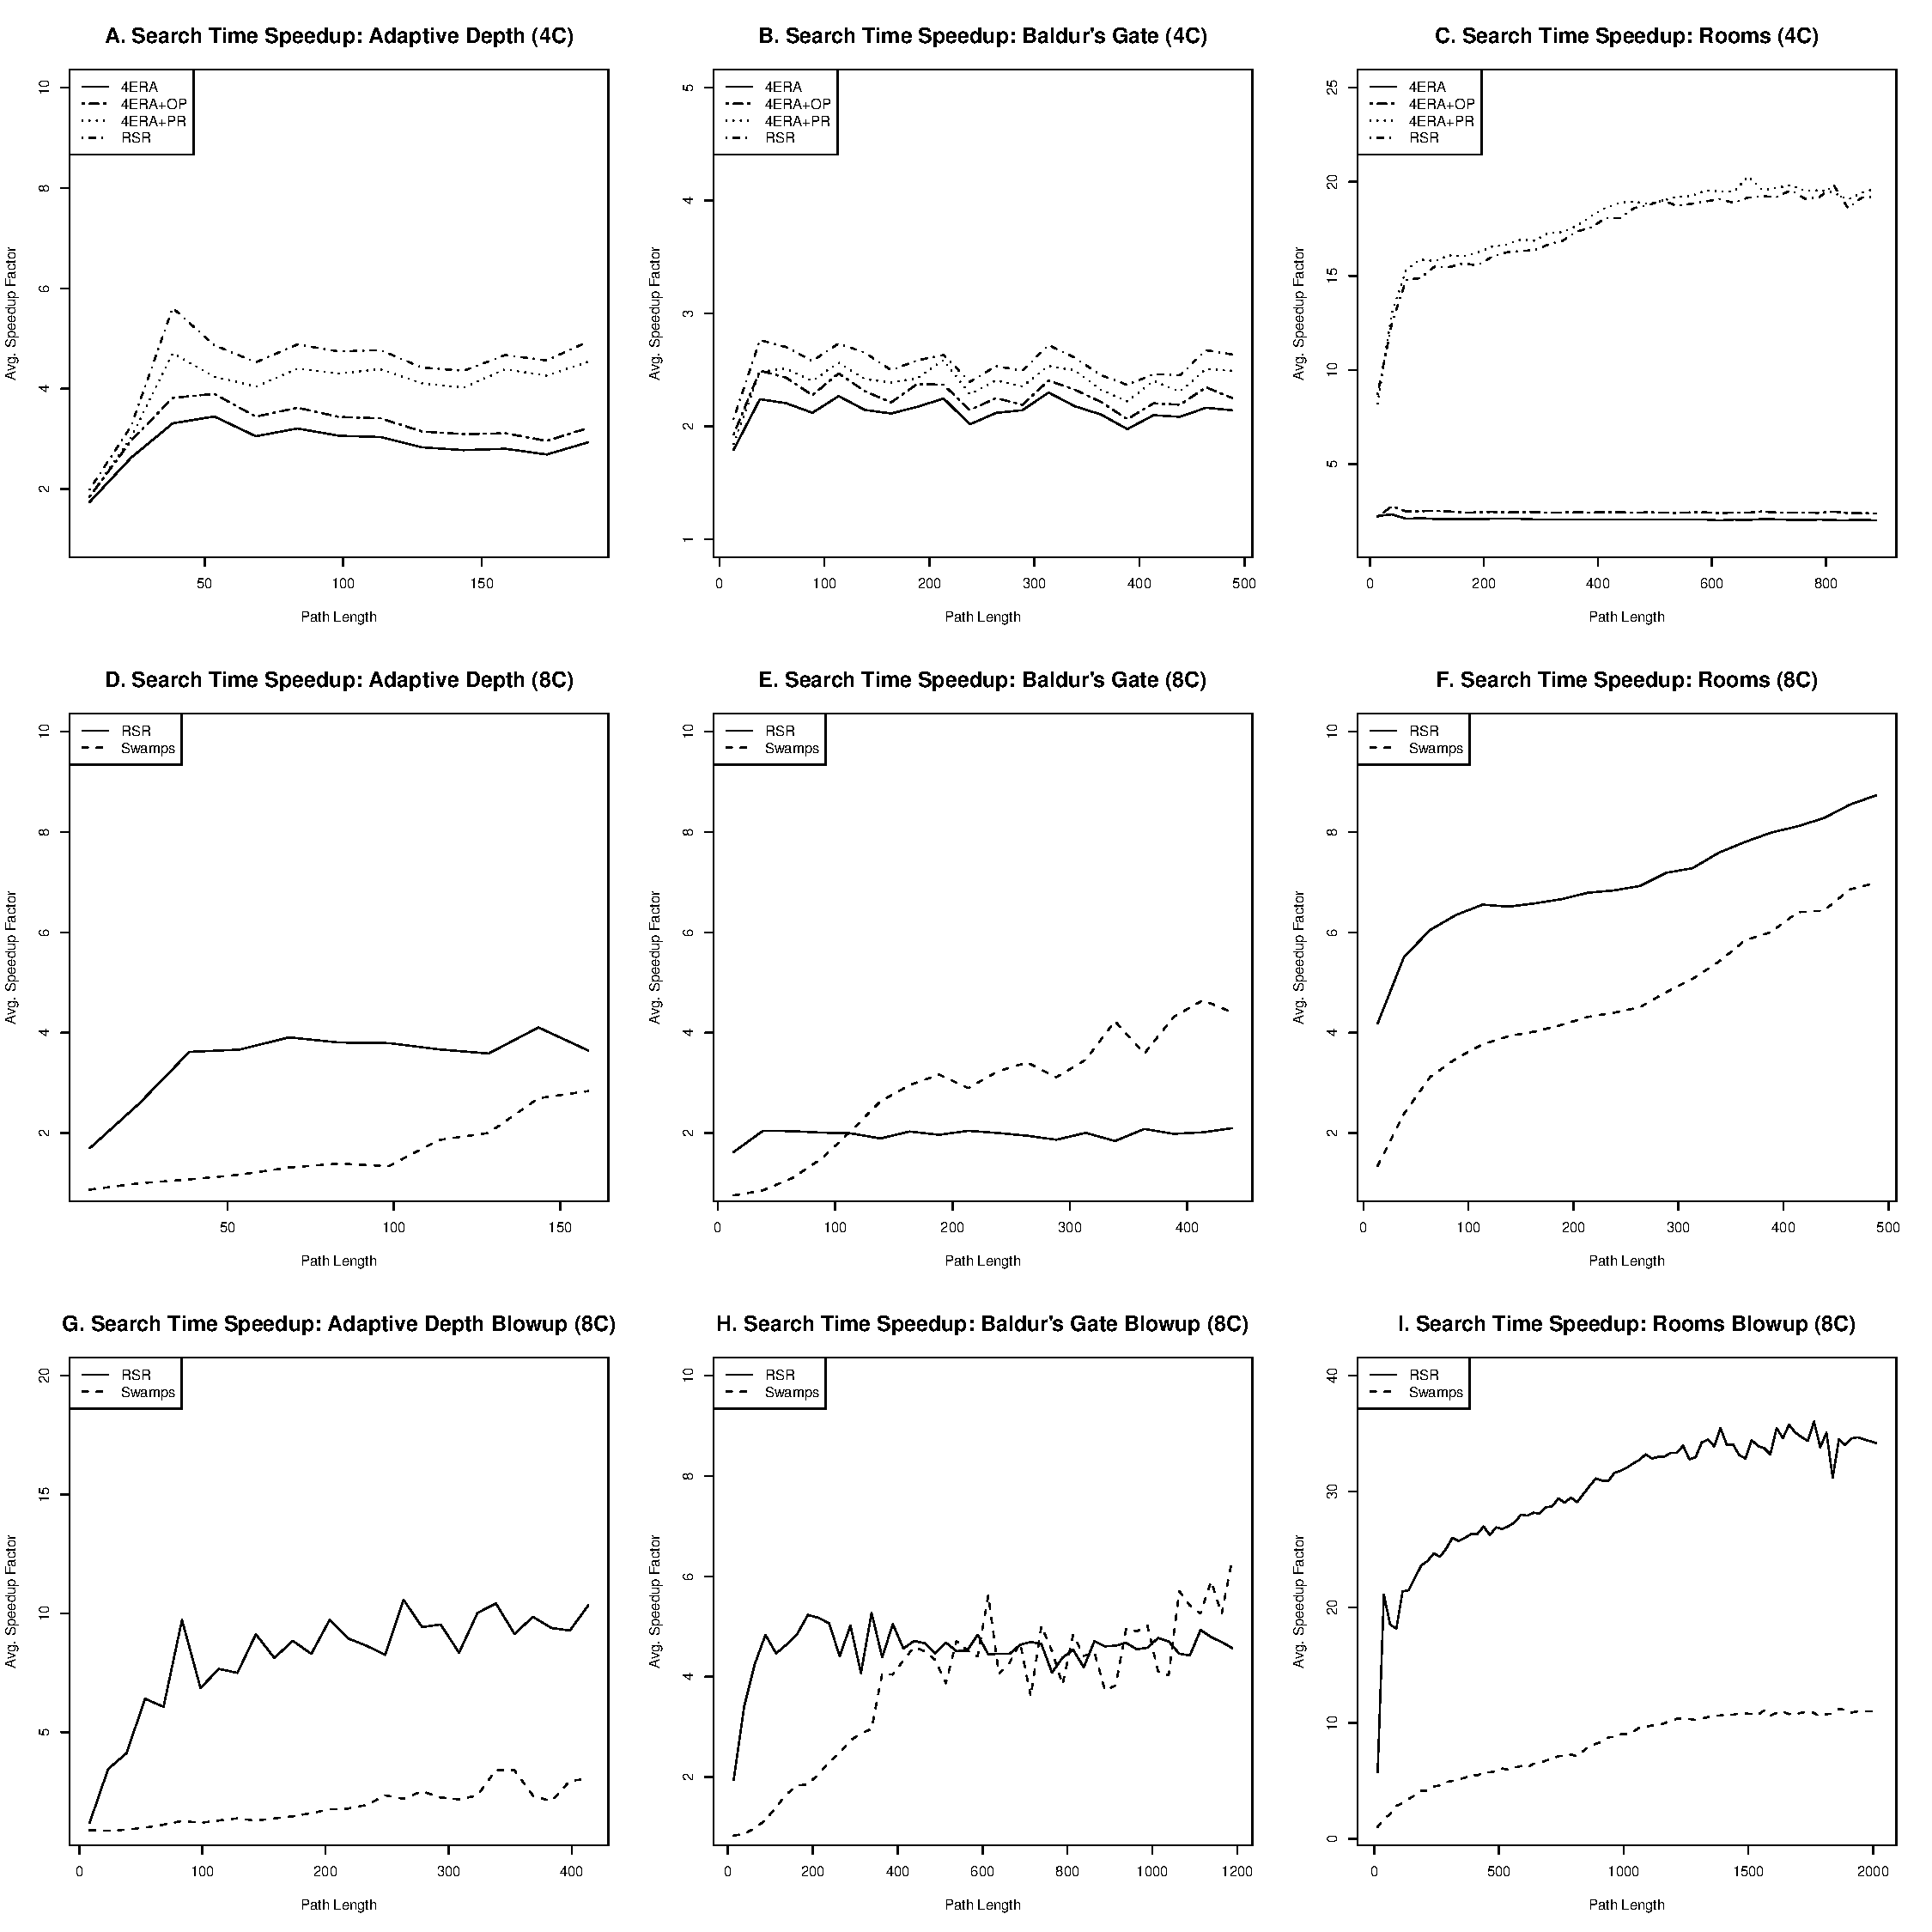
\includegraphics[width=1.95\columnwidth, trim = 10mm 10mm 10mm 0mm]{diagrams/speedup.pdf}
%       \end{center}
%       \caption{Average A* speedup on each of our three benchmarks. 
%		Results are given in terms of nodes expanded and search time.}
%\label{fig-speedup}
%\end{figure*}

Our main results are given in Table \ref{table-graphsize} and Table
\ref{table-speedup}.
%and Figure \ref{fig-speedup}.
We will briefly introduce each and then discuss them in the context
of our three benchmarks.
\par
Table \ref{table-graphsize} measures the size of our modified grid maps.
We give average figures for the number of nodes and number of edges
as a proportion of the total number of nodes and edges found in the 
unmodified grid maps from each benchmark. 
Table \ref{table-speedup} meanwhile shows the average speedup experienced
by A* when running on our modified grid maps as compared to the
original.  We measure speedup in terms of node expansions and search
times.  For example, a search time speedup of 2.0 is twice as fast and
a node expansion speedup of 2.0 indicates 50\% fewer nodes were expanded.
For comparison, we also summarise results on 8-connected maps previously published in \cite{pochter10}.
That work describes a similar algorithm to ours which breaks symmetries by identifying ``Swamps'' --
areas that do not have to be searched because crossing them could not improve the length of any path.
 
\input speedup_table

\textbf{Adaptive Depth:}
The maps in this benchmark were generally favourable for our decomposition algorithm. 
Table \ref{table-graphsize} shows that in the 4-connected case our modified maps contain 
25\% as many nodes and 28\% as many edges, on average, compared to the original unmodified maps.
When we look at the 8-connected case we observe the same reduction in the number of nodes however there is now almost a
doubling in the number of edges.
This increase, which is expected, is due to the high number of edges required to optimally connect nodes on opposite sides of 
each empty room. 
Despite this, the overall savings in graph size are substantial and we achieve a significant speedup.
Table \ref{table-speedup} shows that on 4-connected maps A* runs 4.5 times faster on average and expands 4.4 times fewer nodes.
When we turn our attention to 8-connected maps we see that 4.7 times fewer nodes were expanded but the average
search time was improved by only 3.5 times on average.
This difference is directly attributable to the linear branching factor which results when we apply our decomposition
technique to this domain. 
The effectiveness of each of our Fast Node Expansion and Perimeter Reduction strategies in mitigating this problem can
be clearly seen: without either, A* runs only 1.95 times faster than otherwise. 
\par
\textbf{Baldur's Gate:}
The maps in this benchmark have a distinctive 45 degree orientation which makes it difficult to decompose traversable
areas into rectangular rooms. 
In the 4-connected case we produced grid maps which contain between 49\% as many nodes and 54\% as many
edges, on average, when compared to the original unmodified maps.
However we observed a standard deviation of approximately 11\% associated with these results, indicating a significant level of
variability from one map to another.
On 8-connected maps the savings for nodes are similar but, as expected, we add more edges.
The performance of our decomposition algorithm on this benchmark is reflected in the associated figures measuring search performance:
on 4-connected maps we speed up A* by almost 2.5 times, both in terms of node expansions and search times.
On 8-connected maps we expand almost 2.7 times fewer nodes but improve search times by a more modest factor of 1.8.
We constrast this with the performance of the Swamps based decomposition where A* expands 
2.9 times fewer nodes and search times are improved by a factor of 2.4 on
average.
Although still competitive, we expect that our method could be further improved
given a more effective decomposition algorithm.

\textbf{Rooms:}
The maps in this benchmark are comprised of 32$\times$32 adjacent rectangular rooms. Each room is of size 7$\times$7
and is connected to adjacent rooms by randomly placed entrances.
In the 4-connected case our modified maps contain 7\% as many nodes and 5\% as many
edges, on average, compared to the original unmodified maps.
The smallest maps were achieved using our Perimeter Reduction strategy -- which proved highly effective on this
benchmark.
On 8-connected maps decomposition performance was again very good: our modified maps contain 15\% as many nodes and 13\% as 
many edges as the unmodified originals.
The performance of A* on our modified grid maps was equally encouraging: 
on 4-connected maps we expanded almost 13 times fewer nodes on average and improved search times by a factor of 16.
When dealing with large instances with long path lengths it was not unusual to observe search times up to 20 times
faster.
On 8-connected maps our gains were more modest: A* expands up to 5.8 times fewer nodes on average and runs
up to 6.5 times faster. 
In both cases however our method is competitive with Swamps where we see an
average 6.5 time reduction in node expansions and factor of 7.4 reduction in average search
time.
%The smaller gains, in comparison to the 4-connected case, are directly attributable to the fact that less tiles could be
%pruned. 
%This is in stark contrast to the other two benchmarks where performance was largely limited by having a comparatively
%higher average branching factor than the original unmodified maps.






